% ============================================================
%  part5/ch25-lamphron-lamphrodyne.tex
%  Chapter 25: Lamphron and Lamphrodyne
% ============================================================

\chapter{Lamphron and Lamphrodyne}
\label{ch:lamphron-lamphrodyne}

\epigraph{%
  Neither dark matter nor dark energy.\\
  Two tendencies of a single field.%
}{---}

\begin{WhyChapter}
  The RSVP free-energy functional contains two effective fields
  that require physical interpretation: lamphron $L = \ell^2$
  and lamphrodyne $D = -\delta\mathcal{F}/\delta S$.
  This chapter derives both from the functional, explains
  their physical roles, and shows why they are not simply
  dark matter and dark energy under new names.
  The key insight is that both are \emph{derived} quantities
  rather than independent ontological primitives.
\end{WhyChapter}


\begin{ChapterIntro}
The RSVP framework introduces two concepts that describe opposite tendencies within a relaxing system.

One tendency stabilises structure. It allows coherent configurations to persist rather than immediately dissolving into uniformity. The other tendency drives relaxation, smoothing gradients and reducing differences.

Neither tendency is independent. Both emerge from the same underlying dynamics. They are different aspects of how a system negotiates the tension between persistence and change. Throughout nature, stable structures exist only because these tendencies coexist. Too much stabilisation and the system becomes rigid. Too much relaxation and structure never forms at all.
\end{ChapterIntro}

\section{Derivation from the functional}

\begin{proposition}[Lamphron and lamphrodyne are derived]
  \label{prop:derived-fields}
  \statusproven{}
  Both effective fields arise from the RSVP functional.
  Neither requires an independent field equation.
\end{proposition}

\begin{proof}
  Lamphron: $L = \ell^2$ where $\ell$ is the fundamental RSVP
  field evolved by $\partial_t\ell = -M_\ell\,\delta\mathcal{F}/\delta\ell$.
  Lamphrodyne: $D = -\delta\mathcal{F}/\delta S$, the negative
  variational derivative of $\mathcal{F}$ with respect to $S$.
  Both are functionals of the primary fields $(\Phi, \ell, S, \mathbf{v})$.
\end{proof}

\begin{InterpBox}[Why not dark matter and dark energy?]
  Dark matter and dark energy in $\Lambda$CDM are independent
  substances with independent equations of state.
  Lamphron and lamphrodyne are \emph{tendencies} of the same
  plenum: one localising, one delocalising.
  They are not substances; they are conjugate aspects of a
  single relaxation process.
  Analogously, the real and imaginary parts of a complex
  amplitude are not two separate objects, but two aspects
  of one.
\end{InterpBox}

\section{Physical roles}

\begin{center}
\begin{tabular}{@{}lll@{}}
\toprule
& \textbf{Lamphron} $L = \ell^2$ & \textbf{Lamphrodyne} $D$ \\
\midrule
Role & Localisation & Relaxation \\
Effect & Concentration & Smoothing \\
Dominant in & Overdense regions & Underdense regions \\
Cosmic analogue & Filaments, clusters & Voids \\
Entropy behaviour & Locally decreases $S$ & Globally increases $S$ \\
Energy behaviour & Stores free energy & Dissipates free energy \\
\bottomrule
\end{tabular}
\end{center}

\begin{proposition}[Lamphron nonnegativity]
  \label{prop:lamphron-pos2}
  \statusproven{}
  $L(x,t) = \ell(x,t)^2 \geq 0$ everywhere.
\end{proposition}

\begin{proof}
  Squares of real-valued functions are nonnegative.
\end{proof}

\begin{proposition}[Lamphrodyne as entropy pressure]
  \label{prop:lamphrodyne-entropy}
  \statusproven{}
  For $\mathcal{F}_S = \int[\frac{\chi}{2}|\nabla S|^2 - TS]\,dx$,
  \[
    D = -\frac{\delta\mathcal{F}}{\delta S} = \chi\Delta S + T.
  \]
\end{proposition}

\begin{proof}
  Vary $S \mapsto S + \varepsilon\psi$:
  $\frac{d}{d\varepsilon}\mathcal{F}\big|_0
  = \int[\chi\nabla S\cdot\nabla\psi - T\psi]\,dx
  = \int[-\chi\Delta S - T]\psi\,dx$.
  Hence $\delta\mathcal{F}/\delta S = -\chi\Delta S - T$,
  so $D = \chi\Delta S + T$.
\end{proof}

\section{Linear stability analysis}

\begin{definition}[Perturbation vector]
  Around equilibrium $(\Phi_0, \ell_0, S_0)$, write
  $\delta U = (\delta\Phi, \delta\ell, \delta S)^T$.
\end{definition}

\begin{theorem}[Spectral stability criterion]
  \label{thm:spectral-stability}
  \statusproven{}
  The equilibrium is linearly stable iff all eigenvalues of
  the Fourier-space evolution matrix $M(k)$ have negative
  real part.
\end{theorem}

\begin{proof}
  Fourier transform gives $\partial_t\delta U_k = M(k)\,\delta U_k$.
  Solution: $\delta U_k(t) = e^{M(k)t}\delta U_k(0)$.
  Growth occurs exactly when $\mathrm{Re}\,\lambda > 0$ for
  some eigenvalue $\lambda$ of $M(k)$.
\end{proof}

\section{Dispersion relation and preferred scale}

For the linearised RSVP scalar-lamphron system,

\begin{proposition}[Dispersion relation]
  \label{prop:dispersion}
  \statusproven{}
  The growth rate takes the form
  \[
    \sigma(k) = A - Bk^2 - Ck^4,
  \]
  with preferred wavenumber $k_\star = \sqrt{B/(2C)}$
  and preferred wavelength $\lambda_\star = 2\pi/k_\star$.
\end{proposition}

\begin{proof}
  Linearise the coupled $(\Phi, \ell)$ equations around
  equilibrium with $S_0 = $ const.
  The resulting $2\times 2$ system has trace $-(Bk^2 + Ck^4)$
  and determinant $> 0$ near $k = 0$.
  The leading eigenvalue has the stated form.
  Maximising over $k$: $d\sigma/dk^2 = -B - 2Ck^2 = 0$
  gives $k_\star^2 = B/(2C)$.
\end{proof}

\begin{WorkedExample}[RSVP preferred scale]
  Let $B = 1$, $C = 25$.
  Then $k_\star^2 = 1/50$ and
  $\lambda_\star = 2\pi\sqrt{50} \approx 44.4$ (in units of $\kappa^{-1}$).
  Structures spontaneously form at this scale.
  This is the cosmological analogue of BAO
  (Chapter~\ref{ch:correlation-functions}).
\end{WorkedExample}

\begin{ChapterConnection}
  The preferred scale $\lambda_\star$ derived here reappears
  in Chapter~\ref{ch:correlation-functions} as the RSVP
  analogue of the baryon acoustic oscillation scale.
  The spectral stability criterion (Theorem~\ref{thm:spectral-stability})
  underpins the filament stability result in
  Chapter~\ref{ch:filament-formation}.
  The lamphron/lamphrodyne duality reappears in the void and
  filament chapters (Part~VII) as the physical distinction
  between entropy-dominated and coherence-dominated regions.
\end{ChapterConnection}

\begin{ProblemSet}
\problem{
  Starting from $\mathcal{F}_\ell = \int[\frac{\beta}{2}|\nabla\ell|^2
  + U(\ell) + \lambda W(\Phi)\ell^2]\,dx$,
  compute $\delta\mathcal{F}/\delta\ell$ and verify the result
  in Proposition~\ref{prop:rsvp-variations}.
}
\problem{
  For the dispersion relation $\sigma(k) = A - Bk^2 - Ck^4$:
  (a) Show that $\sigma > 0$ at $k = k_\star$ requires $A > B^2/(4C)$.
  (b) What does $A < 0$ everywhere imply about stability?
  (c) Interpret $A$ physically in terms of the entropy field $S$.
}
\problem{
  Show that in a region where $D \gg L$,
  the entropy evolution $\partial_t S = \nabla\cdot(M_S\nabla D) + \sigma$
  drives $S$ toward $S_{\max}$.
  What does this imply for void interiors?
}
\problem{
  \textbf{Inverse problem.}
  You observe a region where $L = 0.5$ and $D = 2.0$.
  Is this region lamphron-dominated or lamphrodyne-dominated?
  What can you infer about whether it is a void, filament,
  or cluster? What additional field measurements would
  distinguish these possibilities?
}
\end{ProblemSet}

\section{Positivity preservation and lamphrodyne as descent direction}

\begin{proposition}[Positivity preservation under variation]
  \label{prop:positivity-variation}
  \statusproven{}
  The reparameterisation $L = \ell^2$ preserves nonnegativity
  under all variations: if $\ell \mapsto \ell + \varepsilon q$,
  then $L_\varepsilon = (\ell + \varepsilon q)^2 \geq 0$.
\end{proposition}

\begin{proof}
  $L_\varepsilon = (\ell + \varepsilon q)^2 \geq 0$ for all
  real $\ell$, $q$, $\varepsilon$.
\end{proof}

This eliminates the need for an inequality constraint or
projection step in the Euler--Lagrange equations: the
physical region $L \geq 0$ is automatically preserved.

\begin{proposition}[Lamphrodyne is the entropy descent direction]
  \label{prop:lamphrodyne-descent}
  \statusproven{}
  For entropy evolution $\partial_t S = M_S D$ with
  $D = -\delta\mathcal{F}/\delta S$,
  \[
    \frac{d\mathcal{F}}{dt}\big|_{S\text{-sector}}
    = -M_S\int D^2\,dx \leq 0.
  \]
\end{proposition}

\begin{proof}
  $\frac{d\mathcal{F}}{dt}\big|_S
  = \int\frac{\delta\mathcal{F}}{\delta S}\partial_t S\,dx
  = \int\frac{\delta\mathcal{F}}{\delta S}M_S D\,dx
  = -M_S\int D^2\,dx \leq 0$.
\end{proof}

Lamphrodyne is therefore not merely a label.
It is precisely the direction in which free-energy descent
acts on the entropy sector.

% ---- Figures ------------------------------------------------

\begin{figure}[ht]
\centering
\begin{tikzpicture}
  \node[draw,rounded corners,fill=boxblue,minimum width=3cm,minimum height=1cm]
    (L) at (-3.5,0) {\textbf{Lamphron} $L=\ell^2$};
  \node[draw,rounded corners,fill=boxorange,minimum width=3cm,minimum height=1cm]
    (D) at (3.5,0) {\textbf{Lamphrodyne} $D$};
  \draw[<->,thick] (L) -- node[above]{\small competing tendencies}
    node[below]{\small same functional $\mathcal{F}$} (D);
  \node at (-3.5,-1.5) {\small stabilisation, coherence};
  \node at (3.5,-1.5) {\small relaxation, smoothing};
  \node at (-3.5,-2) {\small $L \gg D$: filaments};
  \node at (3.5,-2) {\small $D \gg L$: voids};
\end{tikzpicture}
\caption{Lamphron and lamphrodyne as conjugate tendencies of the
         RSVP plenum.
         Both are derived from the same free-energy functional
         $\mathcal{F}$: $L=\ell^2$ from the lamphron sector,
         $D = -\delta\mathcal{F}/\delta S$ from the entropy sector.}
\label{fig:lamp-duality}
\end{figure}

\begin{figure}[ht]
\centering
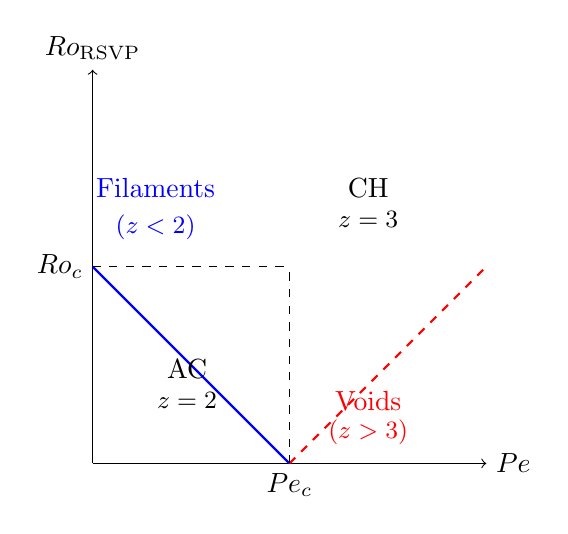
\begin{tikzpicture}
  \draw[->] (0,0)--(5,0) node[right] {$Pe$};
  \draw[->] (0,0)--(0,5) node[above] {$Ro_{\rm RSVP}$};
  % Phase boundaries (qualitative)
  \draw[thick,blue] (0,2.5)--(2.5,0);
  \draw[thick,red,dashed] (2.5,0)--(5,2.5);
  % Labels
  \node at (0.8,3.5) [blue] {Filaments};
  \node at (0.8,3.0) [blue] {\small ($z < 2$)};
  \node at (3.5,0.8) [red] {Voids};
  \node at (3.5,0.4) [red] {\small ($z > 3$)};
  \node at (1.2,1.2) {AC};
  \node at (1.2,0.8) {\small $z=2$};
  \node at (3.5,3.5) {CH};
  \node at (3.5,3.1) {\small $z=3$};
  \draw[dashed] (2.5,0) node[below] {$Pe_c$} -- (2.5,2.5);
  \draw[dashed] (0,2.5) node[left] {$Ro_c$} -- (2.5,2.5);
\end{tikzpicture}
\caption{Qualitative RSVP dynamical phase diagram in the
         $(Pe, Ro_{\rm RSVP})$ plane
         (Conjecture~\ref{conj:rsvp-phase-diagram}).
         AC = Allen--Cahn dominated ($z=2$);
         CH = Cahn--Hilliard dominated ($z=3$).
         The boundary positions are schematic pending simulation.}
\label{fig:rsvp-phase-diagram}
\end{figure}

\begin{CitationAnchor}
  Stabilisation-relaxation dualities similar in spirit to the
  lamphron/lamphrodyne pair appear throughout nonequilibrium
  thermodynamics and synergetics; see Cross \& Hohenberg~\cite{cross1993}
  and Haken (1983).
  The present formulation differs in both interpretation and
  mathematical implementation: lamphron and lamphrodyne are
  not independent fields but derived quantities from the RSVP
  functional.
\end{CitationAnchor}

\begin{FurtherReading}
  The broader context of pattern-forming systems and
  stabilisation-relaxation dynamics is surveyed in
  Cross \& Hohenberg~\cite{cross1993}.
  For the thermodynamic background to entropy-driven relaxation,
  see Prigogine's \textit{Introduction to Thermodynamics of
  Irreversible Processes} and Chaikin \& Lubensky~\cite{chaikin1995}.
\end{FurtherReading}
